\documentclass[../stats.tex]{subfiles}
\graphicspath{{\subfix{../figures/}}}
\begin{document}
\chapter{Collecting Data}
\section{Planning a Study}
In order to better understand the characteristics of a population, statisticians and researchers often use a sample from that population and make inferences based on the summary results from the sample.

Population - the entire group we want information about. 

A population can be huge like ``all women'' or small like ``top 200 grossing movies in 2023.''

Sample - a part of the population we actually examine.

The size of the sample can vary and depends on several factors we will examine through the course.
\begin{center}
    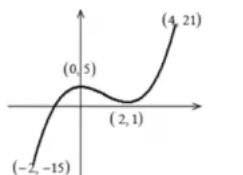
\includegraphics[width=0.8\textwidth]{3.1.1.PNG}
\end{center}

Census - collects data from every individual in the population.

The way we collect data influences what we can and cannot say about a population.

Observation Study - observes individuals and measures variables of interest but does not attempt to influence the responses.
\begin{itemize}
    \item In an observational study, treatments are not imposed 
    \item Investigators examine data for a sample of individuals (retrospective) or follow a sample of individuals into the future collecting data (prospective) in order to investigate a topic of interest about the population.
    \item A sample survey is a type of observational study that collects data from a sample in an attempt to learn about the population which the sample was taken
\end{itemize}

Experiment - deliberately imposes some treatment on individuals to measure their responses.
\begin{itemize}
    \item We will discuss experiments in a later topic in this unit.
\end{itemize}

For now, let's discuss the various ways we plan an observational study.

It is only appropriate to make generalizations about a population based on samples that are randomly selected or otherwise representative of that population.
\begin{itemize}
    \item A sample is only generalizable to the population from which the sample was selected.
    \begin{itemize}
        \item For example, if you poll a sample of women asking about their shopping habits, you cannot take that result and apply it to men, since they were not represented in the sample that was taken.
    \end{itemize}
    \item It is not possible to determine casual relationships between variables using data collected in an observational study.
    \begin{itemize}
        \item While we observe variables and gather data in an observational study, we cannot make inferences between the variables. As long as it is a well-designed observational study, we can only apply the findings from the sample to the population.
    \end{itemize}
\end{itemize}

Because we make inferences about a population from the sample, it is very important that the sample is collected appropriately and that is it representative of the population being studied.

Convenience Sample:
\begin{itemize}
    \item Definition: Uses subjects that are readily avaliable.
    \item Advantage: Easy and less costly to collect 
    \item Disadvantage: Not representative of the population 
    \item Example: In order to get an idea of how students think of the new school policy, the principal stands outisde the library and asks a few students their opinions.
\end{itemize}

Voluntary Response Sample:
\begin{itemize}
    \item Definition: A sample obtained by allowing subjects to decide whether or not to respond.
    \item Advantage: Easy to collect 
    \item Disadvantage: Overrepresents people with strong opinions 
    \item Example: After the State of the Union speech, ABC tells its audience to call a 1-900-555-1234 if they thought the speech was good and 1-900-555-7890 if they thought the speech was bad (there is a \$0.50 charge for the call).
\end{itemize}

Simple Random Sample (SRS)
\begin{itemize}
    \item Definition: Consists of $n$ individuals from the population chosen in such a way that every set of $n$ individuals has an equal chance in the sample selected.
    \item Advantage: Easy to accomplish using a table of random digits; likely to produce samples that are good representatives of the population 
    \item Disadvantage: Cost or time could be an issue 
    \item Example: In order to determine how happy students are with their education at a high school, the principal assigns each student a number from 1 to 1230 and then uses a random number generator to choose 50 numbers between 1 and 1230. He then surveys all the students with the chosen numbers.
\end{itemize}

Stratified Random Sampling 
\begin{itemize}
    \item Definition: Divide the population into groups of similar individual (strata) then select an SRS within each strata. Combine the SRSs from each strata to form your full sample.
    \item Advantage: Can produce more exact information (especially in large populations) by taking advantage of the fact that individuals in the same strata are similar to one another 
    \item Disadvantage: Not appropriate unless strata are easily defined 
    \item Example: In order to get a better idea of what a high school's athletes thought about homecoming last year, the director divides all the athletes into the teams they play for, and then selects a random sample from each sports team. His full sample consists of aggregating the random samples from each team.
\end{itemize}

Cluster Sampling: 
\begin{itemize}
    \item Definition: Divide the population into sectors (clusters) then randomly choose a few of those clusters. Each member of the cluster becomes your sample.
    \item Advantage: Don't need a list of entire population 
    \item Disadvantage: More variability between samples depending on how clusters are determined.
    \item Example: A psychologist at the University of Texas collects a sample by first dividing up the students into their respective schools (engineering, nursing, arts and sciences) then by the departments that their major is in, and then she selects a few departments that their major is in, and then she selects a few departments at random and surveys every student within those chosen departments.
\end{itemize}

Systematic Random Sampling 
\begin{itemize}
    \item Definition: Randomly select an arbitrary starting point and then select every $k$th member of the population.
    \item Advantage: Every member has an equal probability of being selected.
    \item Disadvantage: Not every sample of size $n$ has an equal chance of being selected.
    \item Example: HP selects every 200th computer off the assembly line and inspects it for quality control.
\end{itemize}

When an item from a population can be selected only once, this is called without replacement. When an items from the population can be selected more than once, this is called with replacement.

Samples are biased if they are systematically not representative of the desired population.
\begin{itemize}
    \item Bias occurs when certain responses are systematically favored over others.
\end{itemize}

Voluntary Response: When a sample is comprised entirely of volunteers or poeple who choose to participate, the sample will typically not be representative of the population (voluntary response bias).
\begin{itemize}
    \item Example: A radio talk show host asks listeners to call in with their opinions of making wearing masks in public space mandatory.
\end{itemize}

Undercoverage: Occurs when some groups in the population are left out of the process of choosing a sample.
\begin{itemize}
    \item Because they are generally fearful of government intrusion, many immigrants from Latin America did not return their census questionaire during the 1990 census.
\end{itemize}

Non-response: Occurs when an individual chosen for a sample can't be contacted or refuses to respond. Non-response is a big problem in mail surveys.
\begin{itemize}
    \item Example: Our administration sends out 100 survey questions to a sample of parents in order to gage their attitudes towards returning to school in 2020. Only 23 respond.
\end{itemize}

Response Bias - bias caused by the behavior of the respondent or interviewer.

Untruthful Answers: people give untruthful answers for several reasons..
\begin{enumerate}
    \item Sensitive Questions: How often do you drink alcohol?
    \item Socially Acceptable Answers: Do you use corporal punishment with your children?
    \item Interview Bias: One year after the Detroit race riots of 1967, interviewers asked a sample of black residents in Detroit if they felt they could trust most white people, some white people, or none at all. When the interviewer was white, 35\% answered ``most'', when the interviewer was black, 7\% answered ``most''.
\end{enumerate}

Ignorance: people will give silly answered just so they appear to know something about the subject.
\begin{itemize}
    \item Example: In a study, educators were asked how they would rank Princeton's undergraduate business program. In every case, it was rated among the top 10 departments in the country, even though Princeton doesn't offer an undergraduate business major.
\end{itemize}

Lack of Memory: giving a wrong answer simply because respondent doesn't remember the correct answer.
\begin{itemize}
    \item Example: Students were asked to report their grade point averages. Researches then determined the actual GPA's. Over 17\% of the students reported a GPA that was .4 or more above their actual average, and about 2\% reported a GPA more than .4 below their actual GPA. (most inflated their GPA's!) 
\end{itemize}

Timing: When a survey is taken can have an impact on the answers 
\begin{itemize}
    \item Example: In January, the National Football League reported a poll that revealed football as the nation's favorite sport (this is at the time of the Super Bow;)
\end{itemize}

Phrasing: Subtle differences in phrasing make large differences in the results.

Example:
\begin{itemize}
    \item Should the president hae the line-item veto to eliminate waste? 97\% said ``yes'' 
    \item Should the president have the line-item veto? 57\% said ``yes''
\end{itemize}

When drawing a sample, two types of errors may occur:

Sampling Error: The difference between a sample result and the true population result. This error results from chance variation.

Example: Place 50 red and 50 green balls in a bag. Mix the balls thoroughly and randomly sample 30 balls. In your sample you find that 12 balls are red and 18 are green. Your sample result is different than the true population ratio of 1 to 1. The difference is due to sampling error.
Virtually any experiment involving a sample will have sampling error. We can minimize sampling error through various statistical techniques, the most obvious is to increase sample size.

Non-sampling error: Occurs when the sample data is incorrectly collected, recorded, or analyzed. Usually occurs when the sample is selected in a non-random fashion.

Example: In order to gage student opinion on a new grading policy, an administrator stands outside the library during common time and asks a sample of 50 students if they agree with the new policy. The administrator finds that 25 out 
of the 50 students sampled agree with the new policy. When the entire student body is asked for their opinion, however, the results were 30\% in factor 70\% against. The difference between the sample percentage and the true population 
percentage is due to non-sampling error, because the sample was collected in such a way that a lot of bias was involved (convenience sampling).


\section{Selecting a Random Sample}
The Hat Method 
\begin{itemize}
    \item This is a classic description of an SRS that can be used on the AP exam to describe selecting a random sample but it is rarely done in practice due to it being being so time consuming.
    \item Script: ``Write down all the names or numbers on their own slip of paper. Then put all the pieces of paper into a hat, mix well in-between selections, and pull out the desired amount of slips (mention with or without replacement)''
\end{itemize}

Calculator - Random Number Generator 
\begin{itemize}
    \item MATH - PROB - 5:randInt(lower, upper, n)
    \item Can be used to describe on the AP Exam but not really used for ``doing'' random samples on the AP Exam because there is no way to ``check'' for it.
    \item In practice, computer generated numbers are the least time consuming.
    \item If using this method, make sure you ``seed'' your calculator, otherwise everyone will get the same ``random numbers''.
    \begin{itemize}
        \item MMDDYYYY - STO$\rightarrow$ - MATH - PROB - 1:rand-ENTER
    \end{itemize}
\end{itemize}

Random Digit Table 
\begin{itemize}
    \item Given as a long string of digits 0-9 within the question. The digits are grouped in 5s to make it easier to read but it has no significant meaning.
\end{itemize}
\begin{center}
    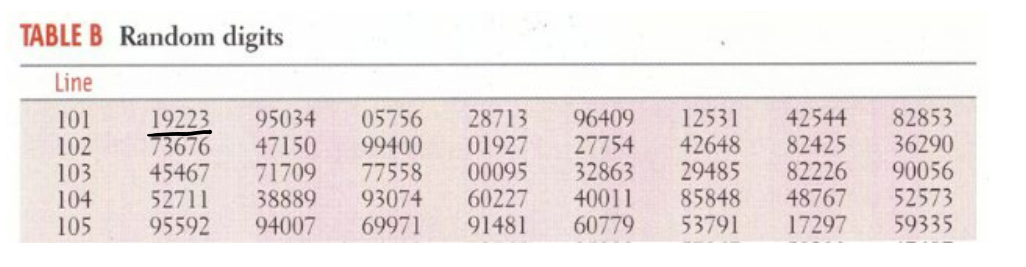
\includegraphics[width=0.8\textwidth]{3.2.1.PNG}
\end{center}

Choosing SRS with a Random Digit Table 
\begin{enumerate}
    \item Label: Assign a number label to every individual in the population.
    \item Random Digits: Start at the very first number and identify how many digits you will take at a time.
    \item Stop: Indicate when you should stop sampling (toss out repeated numbers or numbers out of your range).
    \item Identify Sample: Use the random numbers to identify subjects to be selected from your population. This is your sample!
\end{enumerate}

\begin{example}
    The school newspaper is planning an article on family-friendly places to stay over spring break at a nearby beach town. The editors intend to call 4 randomly chosen hotels to ask about their amenities for families with children. They have an alphabetized list of all 28 hotels in the town.
    Starting at Line 140 (given below), find an SRS of 4 hotels. Describe how you would select your SRS and then collect your sample.
    \begin{center}
        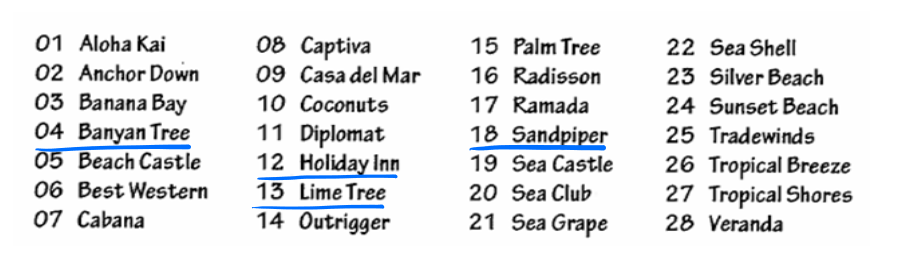
\includegraphics[width=0.8\textwidth]{3.2.2.PNG}
    \end{center}
    \begin{center}
        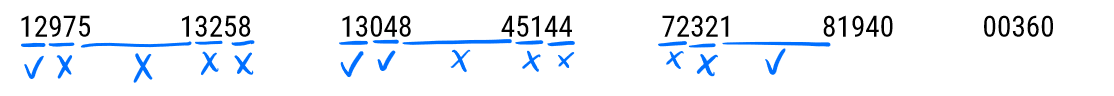
\includegraphics[width=0.8\textwidth]{3.2.3.PNG}
    \end{center}
    \begin{enumerate}
        \item Each hotel is given a number 01 to 28.
        \item Choose 2 digits at a time. If the number is 01-28, it will represent a hotel in the sample.
        \item Ignore numbers 29-99 and repeats. Repeat process until 4 hotels are chosen.
        \item The checkmarks in the image are those to include in the sample, and the x's are skips.
    \end{enumerate}

    The four hotels are 04, 12, 13, and 18.
\end{example}

Observational Study: Observes individuals and measures variables of interest but does not attempt to influence the response.

Experiment: Deliberately imposes some treatment on individuals to measure their responese.

Experimental Unit: the things on which the experiment is done 

Subjects: experimental units that are human beings 

Treatment: a specific experimental condition applied to the units 

\begin{example}
    Are the following scenarios an experiment or an observational study? Explain your answer.

    (a) A medical team examines the records of 5 large hospitals and compares the survival times of those cancer patients who had surgery versus those who had chemotherapy.

    Observational Study - medical team did not impose any treatments 

    (b) In a gym class, the effect of exercise on blood pressure is studied by requiring that half of the students walk a mile each day while the other students run a mile each day.

    Experiment - treatments are running or walking a mile.

    (c) The relationship between weights of bears and their lengths is studied by measuring bears that have been anesthetized.

    Observational Study - weights and lengths are recorded, no treatments 

    (d) People who smoke are asked to halve the number of cigarettes consumed each day so that any effect on pulse rate can be measured.

    Experiment - treatment is halving cigarettes
\end{example}

\begin{example}
    Determine if it is an observational study or an experiment, and then identify the explanatory and response variables in each situation.

    (a) One effect of alcohol is a drop in body temperature. To study this effect, researchers give several amounts of alcohol to mice, and then measured the change in each mouse's body temperature.

    Experiment, explanatory: amount of alcohol, response: body temperature 

    (b) A study is done to try and find the correlation between verbal and math SAT scores. The scientist wants to use the verbal score to predict the math score.

    Observational Study, explanatory: verbal SAT score, response: math SAT score 

    (c) Some breast cancer patients were given each a new treatment. The patients were closely followed to see how long they lived following surgery.

    Experiment, explanatory: ``new treatment'', response: length of life 

    (d) To find out how well a child's height predicts their age a study was done where they measured the heights of a group of children at age 6, wait until they are 16 and then measure their heights again.

    Observational study, explanatory: height, response: age
\end{example}

\section{Experimental Design}
Two advantages of an experiment over an observational study:
\begin{enumerate}
    \item We can study the specific factors we are interested in while controlling the effects of lurking variables.
    \item Experiments also allow us to study the combined effects of several factors.
\end{enumerate}

How to design an experiment 
\begin{itemize}
    \item Factor: The explanatory variables in an experiment
    \item Level: the various groups the factors take 
\end{itemize}

For example, if an experiment compared the drug doses 50 mg, 100 mg, and 150 mg, then the factor ``drug dosage'' would have three levels: 50 mg, 100 mg, and 150 mg 

Prinicples of Experimental Design 
\begin{enumerate}
    \item Comparison 
    \begin{itemize}
        \item We want to make sure we are using a design that compares two or more treatments 
        \item We need to make sure the groups we are comparing don't differ greatly before our experiment begins or bias can result.
    \end{itemize}
    \item Randomization 
    \begin{itemize}
        \item The most important element of any experiment. It must be incorporated either in the selection process of experimental units and/or the distribution of experimental units into treatment and control groups.
        \item You can use your calculator (random number generator), random digit table, the hat method, or flipping a coin to randomize an experiment.
        \item Randomization produces groups of experimental units we expect to be similar in all respects before treatment is applied. Therefore, measured differences must be due either to treatment or by change of random assignment.
    \end{itemize}
    \item Control 
    \begin{itemize}
        \item Control group is treated identically in all respects to the group receiving the treatment except that the members of the control group do not receive the treatment.
        \item The control group is our baseline and our experimental group has only one thing changed - the explanatory variable.
        \item This reduces variability in the reponse variable. If one group is controlled, we would expect their responses to be controlled as well.
    \end{itemize}
    \item Replication 
    \begin{itemize}
        \item Use enough experimental units in each group so that any difference in the effects of the treatments can be distinguished from chance differences between groups.
        \item Even with control, natural variability occurs among experimental units.
        \item We would like to see units within a treatment group responding similarly to one another, but differently from units in other treatment groups (then we can be sure that the treatment is responsible for the differences).
        \item If we assign many individuals to each treatment group, the effects of chance (and individual differences) will average out.
    \end{itemize}
\end{enumerate}

Experimental Terms 
\begin{itemize}
    \item Placebo: treatment designed to have no therapeutic value 
    \item Placebo Effect: subjects receiving the placebo have a response that is similar to what we would expect from the treatment 
    \item Single Blind: subject does not know what treatment they are receiving 
    \item Double Blind: subject and administrator do not know who receives the treatment 
\end{itemize}

The design of an experiment is crucial. Experiments are designed with the purpose of isolating the effect of the treatment on the response variable and removing any confounding effects.
\begin{itemize}
    \item In a poorly designed experiment, it might be difficult to tell if the explanatory variable causes a change or if it was another variable that wasn't measured 
    \item Confounding variables are variables that might affect the outcome, but we did not control or account for them in our experiment.
\end{itemize}

One way to remove the effect of any confounding variable is to randomly assign subjects to the treatment or control group. This allows for any possible bias in the population to be evenly spread among the treatment and control groups.
Sometimes instead of relying on randomization to make groups as even as possible we actually force the groups to be similar.

An extraneous variable is one that is not an explanatory variable in the study but is thought to affect the response variable. There are two types of extraneous variables present in studies:

Confounding variable refers to another variable that may affect the response and is in some way tied together with the factor under investigation. It leaves us unable to tell which of the two variables (or perhaps some interaction) caused the observed response.

For example, we plant tomatoes in a garden that's half-shaded. We test a fertilizer by putting it on the plants in the sun and apply none to the shaded plants. Months later the fertilized plants grow more and better tomatoes. Why? 
Well, maybe it's the fertilizer, maybe it's the sun, maybe we need both. We're unable to conclude that the fertilizer works because any effect of fertilizer is confounded with any effect of the extra sunshine.
\begin{center}
    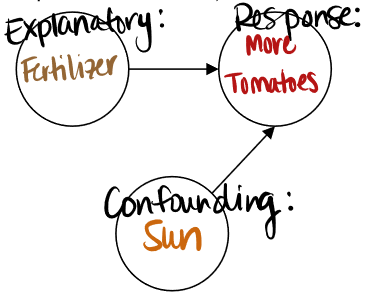
\includegraphics[width=0.5\textwidth]{3.3.1.PNG}
\end{center}

Lurking variable refers to a variable that drives each of the two variables under investigation, making it appear that there's some association between them.

For example, there is a strong association between the number of firefighters who respond to a fire and the amount of damage done. One shouldn't conclude that the firefighters may 
be responsible for the damage; the lurking variable is the size of the fire. 

Lurking variables are the risk we face in sampling and observational studies. In an experiment, though, the factor under consideration isn't being driven by some lurking variable, because we are the ones in control there.
\begin{center}
    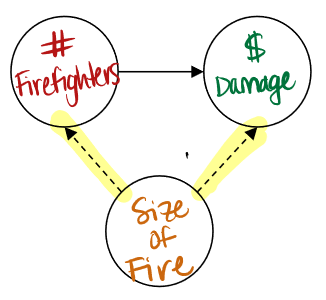
\includegraphics[width=0.5\textwidth]{3.3.2.PNG}
\end{center}

\begin{example}
    State whether the relationship between the two variables involves a lurking or confounding variable.

    (a) Does watching TV make you live longer? Measure the number of television sets per person, $x$, and the average expectancy, $y$, for the world's nation. There is a high positive correlation: nations with many TV sets have high life expectancies. Could we lengthen the lives of people in Rwanda by shipping them TV sets? Justify your answer.

    Lurking variable is money.

    Money pays for food and healthcare (increasing life expectancy). More TVs generally mean more money.

    (b) Do artificial sweeteners cause weight gain? People who use artificial sweeteners in place of sugar tend to be heavier than people who use sugar. Does this mean that artificial sweeteners cause weight gain? Give a more plausible explanation for this association.

    The confounding variable is diet.

    People who use artificial sweeteners could be trying to lose weight so they may be heavier to begin with.
\end{example}

Inference is drawing conclusions beyond the data at hand.

Let's take a look at two different studies:

Study 1: The U.S. Census Bureau carries out a monthly Current Population Survey of about 60,000 households. Their goal is to use data from these randomly selected households to estimate the percent of unemployed individuals in the population.

Study 2: Scientists performed an experiment that randomly assigned 21 volunteer subjects to one of two treatments: sleep deprivation for one night or unrestricted sleep. The experimenters hoped to show that sleep deprivation causes a decrease in performance two days later.
\begin{itemize}
    \item Random selection of individuals allows inference for the population 
    \item Random assignment in an experiment allows inference for cause and effect 
\end{itemize}

For the U.S. Census Bureau, individuals were randomly chosen to participate in the survey. The Bureau would be safe in making an inference about the population.

In the sleep deprivation experiment, subjects were randomly assigned to their treatments. If there is a large difference in the results, then we can assume it is not due to chance variation 
between the groups alone and must be due to sleep deprivation.

Well-designed experiments randomly assign individuals to treatment groups, but most don't select experimental units at random from the larger population, so their findings are limited to just cause and effect.
\begin{center}
    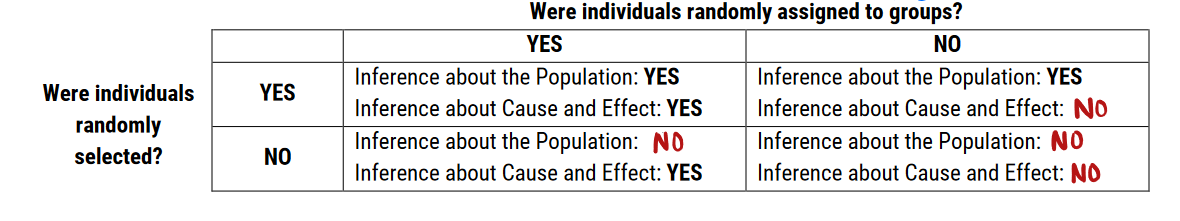
\includegraphics[width=0.8\textwidth]{3.3.3.PNG}
\end{center}

Both random sampling and random assignment introduce chance variation into a statistical study. When performing inference, statisticians use the laws of probability to describe this chance variation.

In some cases, it is not practical or ethical to do an experiment to establish a cause and effect relationship. Consider the following examples:
\begin{itemize}
    \item Does texting while driving increase the risk of having an accident?
    \item Does going to church regularly help people live longer?
    \item Does smoking cause lung cancer?
\end{itemize}

There are laws now that must be followed when dealing with human subjects:
\begin{itemize}
    \item Reviewed by an institutional review board - the board's purpose is ``to protect the right and welfare of human subjects recruited to participate in research activities.''
    \item Informed consent - subjects must be aware of the harm and danger a study could inflict and must be given written permission to participate.
    \item Confidentiality - protect individuals' privacy by keeping their identity separate from their results.
\end{itemize}

Writing up an experiment 
\begin{enumerate}
    \item Determine what type of design is best for your experiment. This will depend on the context of the question.
    \item Diagram your experiment (time permitting).
    \item Tell exactly how you will randomly assign your treatments.
    \begin{itemize}
        \item Random Digit Table 
        \item The Hat Method 
        \item Dice, Coin, or Playing Cards 
    \end{itemize}
    \item Explain exactly what you are comparing once you gather the data 
\end{enumerate}

Completely Randomized Design 
\begin{itemize}
    \item The experimental units are assigned to treatments completely by chance.
    \item Treatment groups and control groups will be about equal in size in a completely randomized design.
    \item There are mathematical reasons for having groups of equal sizes, which we will discuss later.
\end{itemize}

\begin{example}
    Is texting while driving causing accidents? There are 40 students that have volunteered for a study to determine if texting while driving causes more accidents. The county sheriff's department has given a driving simulator to use in the experiment. Design a completely randomized experiment.

    \begin{itemize}
        \item Write each student's name on identical slips of paper and place in a hat.
        \item Select 20 names from the hat without replacement and mixing well in between 
        \item The 20 names selected will receive the treatment - driving while texting 
        \item The remaining 20 students will receive the control - driving while not texting 
        \item Compare the average number of accidents between the two groups 
    \end{itemize}
    \begin{center}
        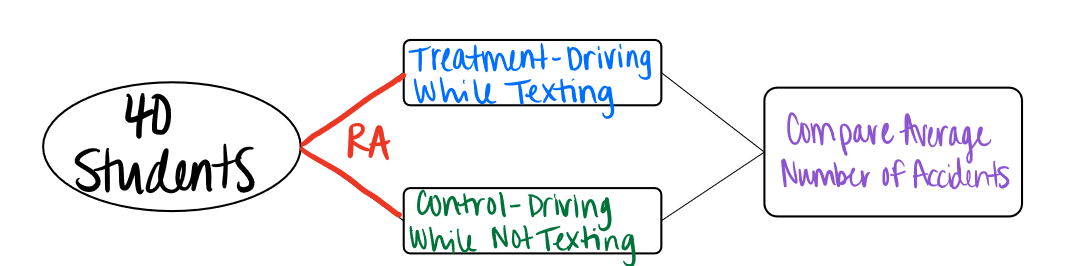
\includegraphics[width=0.8\textwidth]{3.4.1.PNG}
    \end{center}
\end{example}

Randomized Block Design 
\begin{itemize}
    \item When groups of experimental units are similar, it's often a good idea to gather them together in blocks.
    \item Blocking isolates the variability due to the differences between the blocks so that we can see the differences due to the treatments more clearly.
    \item When randomization occurs only within the blocks, we call the design a randomized block design.
    \item Control what you can, block on what you can't control, and randomize to create compatible groups.
\end{itemize}

\begin{example}
    It is brought to a teacher's attention that gender could be another contributing factor to the number of accidents people get into. Design an experiment to address this new information.

    \begin{itemize}
        \item Separate volunteers into two blocks based on gender.
        \item Number males 01-16. Use a random digit table to select 8 unique two digit numbers, ignoring 00 and 17-99.
        \item The 8 names selected will receive the treatment - driving while texting.
        \item The remaining 8 names will receive the control - driving while not texting.
        \item Repeat for females.
        \item Compare the average number of accidents between the two groups within each block.
    \end{itemize}

    \begin{center}
        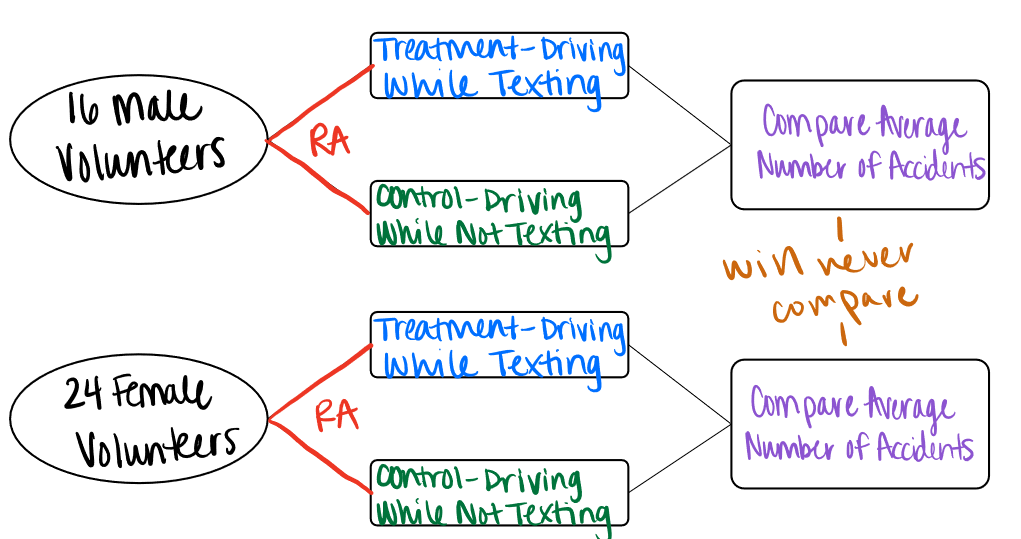
\includegraphics[width=0.8\textwidth]{3.4.2.PNG}
    \end{center}
\end{example}

Matched Pairs Design 
\begin{itemize}
    \item These are experimental designs in which either the same individual or two matched individuals are assigned to receive the treatment and the control.
    \item Often the ``pair'' in a matched pairs design is just one experimental unit which serves as its own control.
    \item In the case where an individual receives both the treatment and the control, the order in which this happens should be random.
\end{itemize}

\begin{example}
    A student now brings up the fact that each student has different driving styles with many other variables that can influence the number of accidents. Design an experiment that would help addres the other variables present for individual drivers.

    \begin{itemize}
        \item Each volunteer will do both treatments.
        \item Randomly assign order of treatments by flipping a coin.
        \item Heads - driving while texting first 
        \item Tails - driving while not texting first 
        \item Perform remaining treatment the next day 
        \item Repeat for other 39 volunteers 
        \item Compare the difference in number of accidents for each of the volunteers 
    \end{itemize}

    \begin{center}
        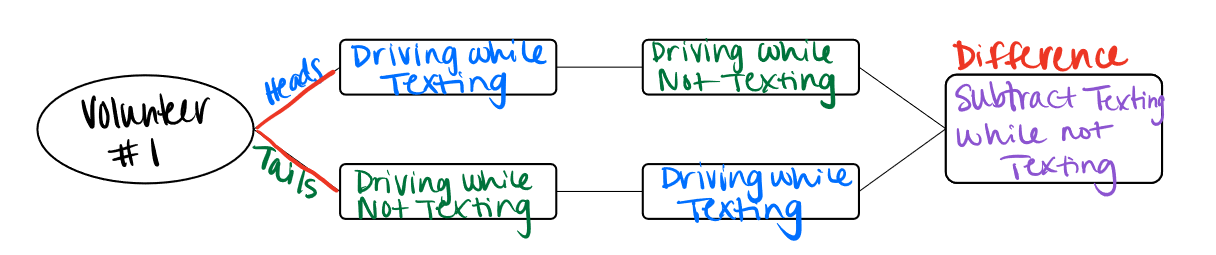
\includegraphics[width=0.8\textwidth]{3.4.3.PNG}
    \end{center}
\end{example}




\end{document}